\documentclass[12pt]{article} 
% Custom definitions
% To use this customization file, insert the line "% Custom definitions
% To use this customization file, insert the line "% Custom definitions
% To use this customization file, insert the line "\input{custom}" in the header of the tex file.

% Formatting

\tolerance=1000
\usepackage[margin=1in]{geometry}


% Packages

% \usepackage{amssymb,latexsym}
\usepackage{amssymb,amsfonts,amsmath,latexsym,amsthm}
\usepackage[usenames,dvipsnames]{color}
\usepackage[]{graphicx}
\usepackage[space]{grffile}
\usepackage{mathrsfs}   % fancy math font
% \usepackage[font=small,skip=0pt]{caption}
\usepackage[skip=0pt]{caption}
\usepackage{subcaption}
\usepackage{verbatim}
\usepackage{url}
\usepackage{bm}
\usepackage{dsfont}
\usepackage{extarrows}
\usepackage{multirow}
% \usepackage{wrapfig}
% \usepackage{epstopdf}
\usepackage{rotating}
\usepackage{tikz}
\usetikzlibrary{fit}					% fitting shapes to coordinates
%\usetikzlibrary{backgrounds}	% drawing the background after the foreground

\usepackage{fancyhdr}

\fancypagestyle{firststyle}{
   \fancyhf{}
   \renewcommand{\footrulewidth}{0.4pt}
   \fancyfoot[L]{\footnotesize This work is licensed under a \href{http://creativecommons.org/licenses/by-nc-nd/4.0/}{Creative Commons BY-NC-ND 4.0 International License}.\\ Jeffrey W. Miller (2015). \textit{Lecture Notes on Bayesian Statistics}. Duke University, Durham, NC.}
}


% \usepackage[dvipdfm,colorlinks,citecolor=blue,linkcolor=blue,urlcolor=blue]{hyperref}
\usepackage[colorlinks,citecolor=blue,linkcolor=blue,urlcolor=blue]{hyperref}
%\usepackage{hyperref}
\usepackage[authoryear,round]{natbib}


%  Theorems, etc.

\theoremstyle{plain}
\newtheorem{theorem}{Theorem}[section]
\newtheorem{corollary}[theorem]{Corollary}
\newtheorem{lemma}[theorem]{Lemma}
\newtheorem{proposition}[theorem]{Proposition}
\newtheorem{condition}[theorem]{Condition}
% \newtheorem{conditions}[theorem]{Conditions}

\theoremstyle{definition}
\newtheorem{definition}[theorem]{Definition}
% \newtheorem*{unnumbered-definition}{Definition}
\newtheorem{example}[theorem]{Example}
\theoremstyle{remark}
\newtheorem*{remark}{Remark}
\numberwithin{equation}{section}



% Document-specific shortcuts
\newcommand{\btheta}{{\bm\theta}}
\newcommand{\bbtheta}{{\pmb{\bm\theta}}}

\newcommand{\commentary}[1]{\ifx\showcommentary\undefined\else \emph{#1}\fi}

\newcommand{\term}[1]{\textit{\textbf{#1}}}

% Math shortcuts

% Probability distributions
\DeclareMathOperator*{\Exp}{Exp}
\DeclareMathOperator*{\TExp}{TExp}
\DeclareMathOperator*{\Bernoulli}{Bernoulli}
\DeclareMathOperator*{\Beta}{Beta}
\DeclareMathOperator*{\Ga}{Gamma}
\DeclareMathOperator*{\TGamma}{TGamma}
\DeclareMathOperator*{\Poisson}{Poisson}
\DeclareMathOperator*{\Binomial}{Binomial}
\DeclareMathOperator*{\NormalGamma}{NormalGamma}
\DeclareMathOperator*{\InvGamma}{InvGamma}
\DeclareMathOperator*{\Cauchy}{Cauchy}
\DeclareMathOperator*{\Uniform}{Uniform}
\DeclareMathOperator*{\Gumbel}{Gumbel}
\DeclareMathOperator*{\Pareto}{Pareto}
\DeclareMathOperator*{\Mono}{Mono}
\DeclareMathOperator*{\Geometric}{Geometric}
\DeclareMathOperator*{\Wishart}{Wishart}

% Math operators
\DeclareMathOperator*{\argmin}{arg\,min}
\DeclareMathOperator*{\argmax}{arg\,max}
\DeclareMathOperator*{\Cov}{Cov}
\DeclareMathOperator*{\diag}{diag}
\DeclareMathOperator*{\median}{median}
\DeclareMathOperator*{\Vol}{Vol}

% Math characters
\newcommand{\R}{\mathbb{R}}
\newcommand{\Z}{\mathbb{Z}}
\newcommand{\E}{\mathbb{E}}
\renewcommand{\Pr}{\mathbb{P}}
\newcommand{\I}{\mathds{1}}
\newcommand{\V}{\mathbb{V}}

\newcommand{\A}{\mathcal{A}}
\newcommand{\C}{\mathcal{C}}
\newcommand{\D}{\mathcal{D}}
\newcommand{\Hcal}{\mathcal{H}}
\newcommand{\M}{\mathcal{M}}
\newcommand{\N}{\mathcal{N}}
\newcommand{\X}{\mathcal{X}}
\newcommand{\Zcal}{\mathcal{Z}}
\renewcommand{\P}{\mathcal{P}}

\newcommand{\T}{\mathtt{T}}
\renewcommand{\emptyset}{\varnothing}


% Miscellaneous commands
\newcommand{\iid}{\stackrel{\mathrm{iid}}{\sim}}
\newcommand{\matrixsmall}[1]{\bigl(\begin{smallmatrix}#1\end{smallmatrix} \bigr)}

\newcommand{\items}[1]{\begin{itemize} #1 \end{itemize}}

\newcommand{\todo}[1]{\emph{\textcolor{red}{(#1)}}}

\newcommand{\branch}[4]{
\left\{
	\begin{array}{ll}
		#1  & \mbox{if } #2 \\
		#3 & \mbox{if } #4
	\end{array}
\right.
}

% approximately proportional to
\def\app#1#2{%
  \mathrel{%
    \setbox0=\hbox{$#1\sim$}%
    \setbox2=\hbox{%
      \rlap{\hbox{$#1\propto$}}%
      \lower1.3\ht0\box0%
    }%
    \raise0.25\ht2\box2%
  }%
}
\def\approxprop{\mathpalette\app\relax}

% \newcommand{\approptoinn}[2]{\mathrel{\vcenter{
  % \offinterlineskip\halign{\hfil$##$\cr
    % #1\propto\cr\noalign{\kern2pt}#1\sim\cr\noalign{\kern-2pt}}}}}

% \newcommand{\approxpropto}{\mathpalette\approptoinn\relax}





" in the header of the tex file.

% Formatting

\tolerance=1000
\usepackage[margin=1in]{geometry}


% Packages

% \usepackage{amssymb,latexsym}
\usepackage{amssymb,amsfonts,amsmath,latexsym,amsthm}
\usepackage[usenames,dvipsnames]{color}
\usepackage[]{graphicx}
\usepackage[space]{grffile}
\usepackage{mathrsfs}   % fancy math font
% \usepackage[font=small,skip=0pt]{caption}
\usepackage[skip=0pt]{caption}
\usepackage{subcaption}
\usepackage{verbatim}
\usepackage{url}
\usepackage{bm}
\usepackage{dsfont}
\usepackage{extarrows}
\usepackage{multirow}
% \usepackage{wrapfig}
% \usepackage{epstopdf}
\usepackage{rotating}
\usepackage{tikz}
\usetikzlibrary{fit}					% fitting shapes to coordinates
%\usetikzlibrary{backgrounds}	% drawing the background after the foreground

\usepackage{fancyhdr}

\fancypagestyle{firststyle}{
   \fancyhf{}
   \renewcommand{\footrulewidth}{0.4pt}
   \fancyfoot[L]{\footnotesize This work is licensed under a \href{http://creativecommons.org/licenses/by-nc-nd/4.0/}{Creative Commons BY-NC-ND 4.0 International License}.\\ Jeffrey W. Miller (2015). \textit{Lecture Notes on Bayesian Statistics}. Duke University, Durham, NC.}
}


% \usepackage[dvipdfm,colorlinks,citecolor=blue,linkcolor=blue,urlcolor=blue]{hyperref}
\usepackage[colorlinks,citecolor=blue,linkcolor=blue,urlcolor=blue]{hyperref}
%\usepackage{hyperref}
\usepackage[authoryear,round]{natbib}


%  Theorems, etc.

\theoremstyle{plain}
\newtheorem{theorem}{Theorem}[section]
\newtheorem{corollary}[theorem]{Corollary}
\newtheorem{lemma}[theorem]{Lemma}
\newtheorem{proposition}[theorem]{Proposition}
\newtheorem{condition}[theorem]{Condition}
% \newtheorem{conditions}[theorem]{Conditions}

\theoremstyle{definition}
\newtheorem{definition}[theorem]{Definition}
% \newtheorem*{unnumbered-definition}{Definition}
\newtheorem{example}[theorem]{Example}
\theoremstyle{remark}
\newtheorem*{remark}{Remark}
\numberwithin{equation}{section}



% Document-specific shortcuts
\newcommand{\btheta}{{\bm\theta}}
\newcommand{\bbtheta}{{\pmb{\bm\theta}}}

\newcommand{\commentary}[1]{\ifx\showcommentary\undefined\else \emph{#1}\fi}

\newcommand{\term}[1]{\textit{\textbf{#1}}}

% Math shortcuts

% Probability distributions
\DeclareMathOperator*{\Exp}{Exp}
\DeclareMathOperator*{\TExp}{TExp}
\DeclareMathOperator*{\Bernoulli}{Bernoulli}
\DeclareMathOperator*{\Beta}{Beta}
\DeclareMathOperator*{\Ga}{Gamma}
\DeclareMathOperator*{\TGamma}{TGamma}
\DeclareMathOperator*{\Poisson}{Poisson}
\DeclareMathOperator*{\Binomial}{Binomial}
\DeclareMathOperator*{\NormalGamma}{NormalGamma}
\DeclareMathOperator*{\InvGamma}{InvGamma}
\DeclareMathOperator*{\Cauchy}{Cauchy}
\DeclareMathOperator*{\Uniform}{Uniform}
\DeclareMathOperator*{\Gumbel}{Gumbel}
\DeclareMathOperator*{\Pareto}{Pareto}
\DeclareMathOperator*{\Mono}{Mono}
\DeclareMathOperator*{\Geometric}{Geometric}
\DeclareMathOperator*{\Wishart}{Wishart}

% Math operators
\DeclareMathOperator*{\argmin}{arg\,min}
\DeclareMathOperator*{\argmax}{arg\,max}
\DeclareMathOperator*{\Cov}{Cov}
\DeclareMathOperator*{\diag}{diag}
\DeclareMathOperator*{\median}{median}
\DeclareMathOperator*{\Vol}{Vol}

% Math characters
\newcommand{\R}{\mathbb{R}}
\newcommand{\Z}{\mathbb{Z}}
\newcommand{\E}{\mathbb{E}}
\renewcommand{\Pr}{\mathbb{P}}
\newcommand{\I}{\mathds{1}}
\newcommand{\V}{\mathbb{V}}

\newcommand{\A}{\mathcal{A}}
\newcommand{\C}{\mathcal{C}}
\newcommand{\D}{\mathcal{D}}
\newcommand{\Hcal}{\mathcal{H}}
\newcommand{\M}{\mathcal{M}}
\newcommand{\N}{\mathcal{N}}
\newcommand{\X}{\mathcal{X}}
\newcommand{\Zcal}{\mathcal{Z}}
\renewcommand{\P}{\mathcal{P}}

\newcommand{\T}{\mathtt{T}}
\renewcommand{\emptyset}{\varnothing}


% Miscellaneous commands
\newcommand{\iid}{\stackrel{\mathrm{iid}}{\sim}}
\newcommand{\matrixsmall}[1]{\bigl(\begin{smallmatrix}#1\end{smallmatrix} \bigr)}

\newcommand{\items}[1]{\begin{itemize} #1 \end{itemize}}

\newcommand{\todo}[1]{\emph{\textcolor{red}{(#1)}}}

\newcommand{\branch}[4]{
\left\{
	\begin{array}{ll}
		#1  & \mbox{if } #2 \\
		#3 & \mbox{if } #4
	\end{array}
\right.
}

% approximately proportional to
\def\app#1#2{%
  \mathrel{%
    \setbox0=\hbox{$#1\sim$}%
    \setbox2=\hbox{%
      \rlap{\hbox{$#1\propto$}}%
      \lower1.3\ht0\box0%
    }%
    \raise0.25\ht2\box2%
  }%
}
\def\approxprop{\mathpalette\app\relax}

% \newcommand{\approptoinn}[2]{\mathrel{\vcenter{
  % \offinterlineskip\halign{\hfil$##$\cr
    % #1\propto\cr\noalign{\kern2pt}#1\sim\cr\noalign{\kern-2pt}}}}}

% \newcommand{\approxpropto}{\mathpalette\approptoinn\relax}





" in the header of the tex file.

% Formatting

\tolerance=1000
\usepackage[margin=1in]{geometry}


% Packages

% \usepackage{amssymb,latexsym}
\usepackage{amssymb,amsfonts,amsmath,latexsym,amsthm}
\usepackage[usenames,dvipsnames]{color}
\usepackage[]{graphicx}
\usepackage[space]{grffile}
\usepackage{mathrsfs}   % fancy math font
% \usepackage[font=small,skip=0pt]{caption}
\usepackage[skip=0pt]{caption}
\usepackage{subcaption}
\usepackage{verbatim}
\usepackage{url}
\usepackage{bm}
\usepackage{dsfont}
\usepackage{extarrows}
\usepackage{multirow}
% \usepackage{wrapfig}
% \usepackage{epstopdf}
\usepackage{rotating}
\usepackage{tikz}
\usetikzlibrary{fit}					% fitting shapes to coordinates
%\usetikzlibrary{backgrounds}	% drawing the background after the foreground

\usepackage{fancyhdr}

\fancypagestyle{firststyle}{
   \fancyhf{}
   \renewcommand{\footrulewidth}{0.4pt}
   \fancyfoot[L]{\footnotesize This work is licensed under a \href{http://creativecommons.org/licenses/by-nc-nd/4.0/}{Creative Commons BY-NC-ND 4.0 International License}.\\ Jeffrey W. Miller (2015). \textit{Lecture Notes on Bayesian Statistics}. Duke University, Durham, NC.}
}


% \usepackage[dvipdfm,colorlinks,citecolor=blue,linkcolor=blue,urlcolor=blue]{hyperref}
\usepackage[colorlinks,citecolor=blue,linkcolor=blue,urlcolor=blue]{hyperref}
%\usepackage{hyperref}
\usepackage[authoryear,round]{natbib}


%  Theorems, etc.

\theoremstyle{plain}
\newtheorem{theorem}{Theorem}[section]
\newtheorem{corollary}[theorem]{Corollary}
\newtheorem{lemma}[theorem]{Lemma}
\newtheorem{proposition}[theorem]{Proposition}
\newtheorem{condition}[theorem]{Condition}
% \newtheorem{conditions}[theorem]{Conditions}

\theoremstyle{definition}
\newtheorem{definition}[theorem]{Definition}
% \newtheorem*{unnumbered-definition}{Definition}
\newtheorem{example}[theorem]{Example}
\theoremstyle{remark}
\newtheorem*{remark}{Remark}
\numberwithin{equation}{section}



% Document-specific shortcuts
\newcommand{\btheta}{{\bm\theta}}
\newcommand{\bbtheta}{{\pmb{\bm\theta}}}

\newcommand{\commentary}[1]{\ifx\showcommentary\undefined\else \emph{#1}\fi}

\newcommand{\term}[1]{\textit{\textbf{#1}}}

% Math shortcuts

% Probability distributions
\DeclareMathOperator*{\Exp}{Exp}
\DeclareMathOperator*{\TExp}{TExp}
\DeclareMathOperator*{\Bernoulli}{Bernoulli}
\DeclareMathOperator*{\Beta}{Beta}
\DeclareMathOperator*{\Ga}{Gamma}
\DeclareMathOperator*{\TGamma}{TGamma}
\DeclareMathOperator*{\Poisson}{Poisson}
\DeclareMathOperator*{\Binomial}{Binomial}
\DeclareMathOperator*{\NormalGamma}{NormalGamma}
\DeclareMathOperator*{\InvGamma}{InvGamma}
\DeclareMathOperator*{\Cauchy}{Cauchy}
\DeclareMathOperator*{\Uniform}{Uniform}
\DeclareMathOperator*{\Gumbel}{Gumbel}
\DeclareMathOperator*{\Pareto}{Pareto}
\DeclareMathOperator*{\Mono}{Mono}
\DeclareMathOperator*{\Geometric}{Geometric}
\DeclareMathOperator*{\Wishart}{Wishart}

% Math operators
\DeclareMathOperator*{\argmin}{arg\,min}
\DeclareMathOperator*{\argmax}{arg\,max}
\DeclareMathOperator*{\Cov}{Cov}
\DeclareMathOperator*{\diag}{diag}
\DeclareMathOperator*{\median}{median}
\DeclareMathOperator*{\Vol}{Vol}

% Math characters
\newcommand{\R}{\mathbb{R}}
\newcommand{\Z}{\mathbb{Z}}
\newcommand{\E}{\mathbb{E}}
\renewcommand{\Pr}{\mathbb{P}}
\newcommand{\I}{\mathds{1}}
\newcommand{\V}{\mathbb{V}}

\newcommand{\A}{\mathcal{A}}
\newcommand{\C}{\mathcal{C}}
\newcommand{\D}{\mathcal{D}}
\newcommand{\Hcal}{\mathcal{H}}
\newcommand{\M}{\mathcal{M}}
\newcommand{\N}{\mathcal{N}}
\newcommand{\X}{\mathcal{X}}
\newcommand{\Zcal}{\mathcal{Z}}
\renewcommand{\P}{\mathcal{P}}

\newcommand{\T}{\mathtt{T}}
\renewcommand{\emptyset}{\varnothing}


% Miscellaneous commands
\newcommand{\iid}{\stackrel{\mathrm{iid}}{\sim}}
\newcommand{\matrixsmall}[1]{\bigl(\begin{smallmatrix}#1\end{smallmatrix} \bigr)}

\newcommand{\items}[1]{\begin{itemize} #1 \end{itemize}}

\newcommand{\todo}[1]{\emph{\textcolor{red}{(#1)}}}

\newcommand{\branch}[4]{
\left\{
	\begin{array}{ll}
		#1  & \mbox{if } #2 \\
		#3 & \mbox{if } #4
	\end{array}
\right.
}

% approximately proportional to
\def\app#1#2{%
  \mathrel{%
    \setbox0=\hbox{$#1\sim$}%
    \setbox2=\hbox{%
      \rlap{\hbox{$#1\propto$}}%
      \lower1.3\ht0\box0%
    }%
    \raise0.25\ht2\box2%
  }%
}
\def\approxprop{\mathpalette\app\relax}

% \newcommand{\approptoinn}[2]{\mathrel{\vcenter{
  % \offinterlineskip\halign{\hfil$##$\cr
    % #1\propto\cr\noalign{\kern2pt}#1\sim\cr\noalign{\kern-2pt}}}}}

% \newcommand{\approxpropto}{\mathpalette\approptoinn\relax}






% Latex Listings language definition/style for Julia
% Source: https://gist.github.com/chi-feng/6589066
%         Github User "chi-feng"
% License: UNKNOWN
% Date accessed: 12/30/2014

% \usepackage{inconsolata} % very nice fixed-width font included with texlive-full
\usepackage{zi4} % EDIT: inconsolata is now accessed through zi4
\usepackage[usenames,dvipsnames]{color} % more flexible names for syntax highlighting colors
\usepackage{listings}
 
\lstset{
basicstyle=\ttfamily, 
columns=fullflexible, % make sure to use fixed-width font, CM typewriter is NOT fixed width
numbers=left, 
numberstyle=\small\ttfamily\color{Gray},
stepnumber=1,              
numbersep=10pt, 
numberfirstline=true, 
numberblanklines=true, 
tabsize=4,
lineskip=-1.5pt,
extendedchars=true,
breaklines=true,        
keywordstyle=\color{Blue}\bfseries,
identifierstyle=, % using emph or index keywords
commentstyle=\sffamily\color{OliveGreen},
stringstyle=\color{Maroon},
showstringspaces=false,
showtabs=false,
upquote=false,
texcl=true % interpet comments as LaTeX
}
 
\lstdefinelanguage{julia}
{
  keywordsprefix=\@,
  morekeywords={
    exit,whos,edit,load,is,isa,isequal,typeof,tuple,ntuple,uid,hash,finalizer,convert,promote,
    subtype,typemin,typemax,realmin,realmax,sizeof,eps,promote_type,method_exists,applicable,
    invoke,dlopen,dlsym,system,error,throw,assert,new,Inf,Nan,pi,im,begin,while,for,in,return,
    break,continue,macro,quote,let,if,elseif,else,try,catch,end,bitstype,ccall,do,using,module,
    import,export,importall,baremodule,immutable,local,global,const,Bool,Int,Int8,Int16,Int32,
    Int64,Uint,Uint8,Uint16,Uint32,Uint64,Float32,Float64,Complex64,Complex128,Any,Nothing,None,
    function,type,typealias,abstract
  },
  sensitive=true,
  morecomment=[l]{\#},
  morestring=[b]',
  morestring=[b]" 
}

\graphicspath{{figures/}}
\def\showcommentary{1}


\title{Chapter 4: Solutions to Exercises}
\author{}
\date{}


\begin{document}
\maketitle
\thispagestyle{firststyle}

\subsection*{Exercise 1}
Because $X_{n+1}\perp X_{1:n}\mid \theta$, we can sample from $X_{n+1}|x_{1:n}$ as follows:
\begin{enumerate}
    \item sample $\theta\sim p(\theta|x_{1:n})$, and then
    \item sample $x_{n+1}\sim p(x_{n+1}|\theta)$.
\end{enumerate}
Since $p(x_{n+1}|\theta) = \N(x_{n+1}|\theta,\lambda^{-1})$, 
step 2 is equivalent to setting $x_{n+1} = \theta + z$, where $z$ is sampled from $\N(0,\lambda^{-1})$, independently.
Thus, the distribution of $X_{n+1}|x_{1:n}$ is the same as the distribution of $\tilde\btheta + Z$, where
\begin{align*}
    & \tilde\btheta\sim p(\theta|x_{1:n})\\
    & Z\sim\N(0,\lambda^{-1})
\end{align*}
independently. Since we know $p(\theta|x_{1:n})=\N(\theta|M,L^{-1})$, where $L = \lambda_0 + n\lambda$ and 
$$M =\frac{\lambda_0\mu_0+\lambda\sum_{i = 1}^n x_i}{\lambda_0+ n\lambda},$$
then by the formula for the sum of independent Normals, we have that
$$ \tilde\btheta + Z \sim \N(M,\,L^{-1}+\lambda^{-1}).$$
Hence, 
$$ p(x_{n+1}|x_{1:n}) = \N(x_{n+1}\mid M,\,L^{-1}+\lambda^{-1}).$$


\subsection*{Exercise 2}

Yum!

\subsection*{Exercise 3}
In some ways, an i.i.d.\ Normal model is appropriate, but in other ways, it is lacking---specifically, the Normal assumption is probably justified, but the i.i.d.\ assumption may not be.  We could reasonably expect the distribution for any given year to be approximately Normally distributed, because annual snowfall represents the sum of the snowfall over many days, and even though there is dependence between the snowfall in successive days, the amount of dependence probably decays quickly enough that the central limit theorem takes effect.  (Note: Technically, it cannot be exactly Normal, since snowfall cannot take negative values---however, when the mean is relatively large compared to the standard deviation, the probability of negative values is exceedingly small.) One possible issue with the i.i.d.\ assumption is that there may be changes in climate over time, causing the amount of snow to increase or decrease (violating the identically distributed assumption). Another possible issue is that there may be dependence between successive years (violating the independence assumption).


\subsection*{Exercise 4}
Based on my prior knowledge before looking at the data, my subjective prior was:
\begin{itemize}
\item $m = 200$ inches (I thought the mean snowfall for each city would be around 15--18 feet)
\item $c = 1$ (I was not certain about this choice of $m$, so I gave it a weight of 1 prior ``sample'')
\item $a = 1/2$ (I was uncertain about the precision, so I chose a weight of 1 prior ``sample'')
\item $b = 80^2 a$ (I thought the standard deviation of the annual snowfall would be around 80 inches)
\end{itemize}
I visualized this prior by making a scatterplot of samples from it, see Figure \ref{figure:snow-prior}. The y-axis is in terms of the standard deviation $\lambda^{-1/2}$, since this is more interpretable than precision. Note that this prior puts non-negligible mass on negative values of the mean snowfall, which is not particularly realistic---it might be better to truncate the prior to make all of the values positive, however, this would probably make very little difference to the posterior. 

\begin{figure}
  \begin{center}
    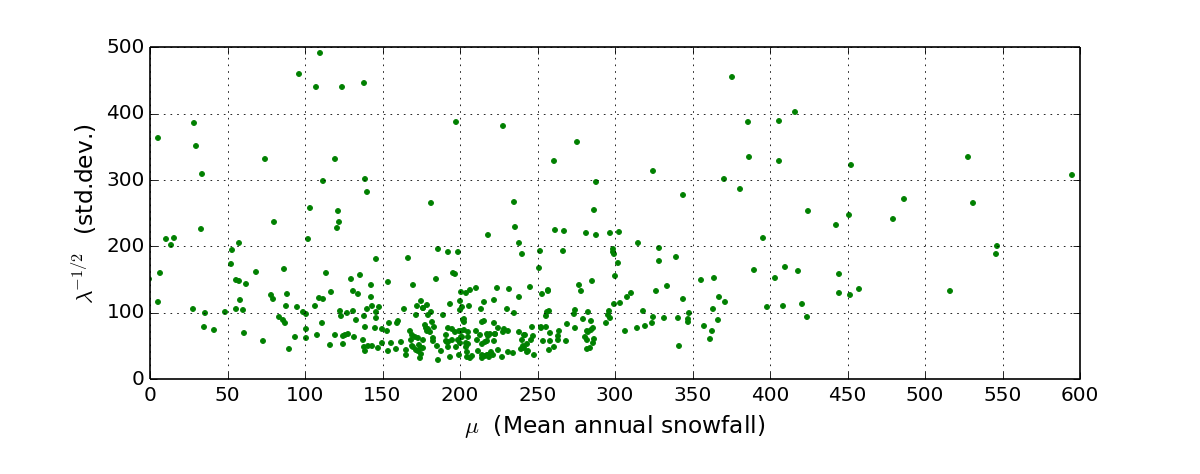
\includegraphics[width=1\textwidth]{code/snow-prior-1.png}
    % Source: Original work by J. W. Miller.
  \end{center}
  \caption{Scatterplot of samples from the prior for the snowfall exercise.}
  \label{figure:snow-prior}
\end{figure}


\begin{figure}
  \begin{center}
    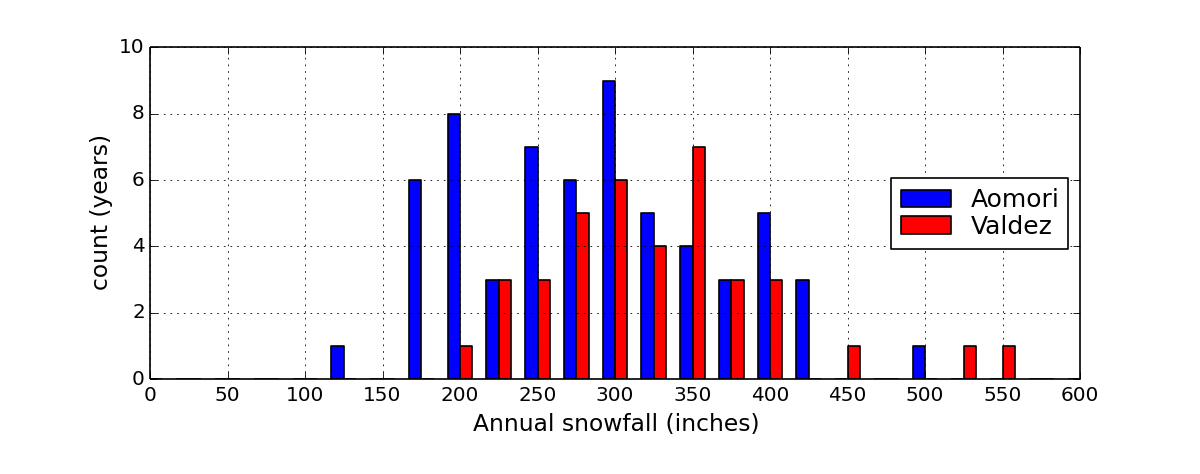
\includegraphics[width=1\textwidth]{code/snow-histogram-1.png}
    % Source: Original work by J. W. Miller.
  \end{center}
  \caption{Histograms of the annual snowfall for Aomori and Valdez.}
  \label{figure:snow-histogram}
\end{figure}


Now, let's visualize the data in a histogram. See Figure \ref{figure:snow-histogram}. From visual inspection, it looks like Valdez has a slight edge---let's see what the posterior says. Using my prior, the posterior parameters are:
\begin{align*}
\text{for Aomori:} & \\
    M & = 285.5\\
    C & = 62\\
    A & = 31\\ 
    B &= 204034\\
\text{for Valdez:} & \\
    M & = 322.2\\
    C & = 39\\
    A & = 19.5\\
    B &= 115204
\end{align*}

\begin{figure}
  \begin{center}
    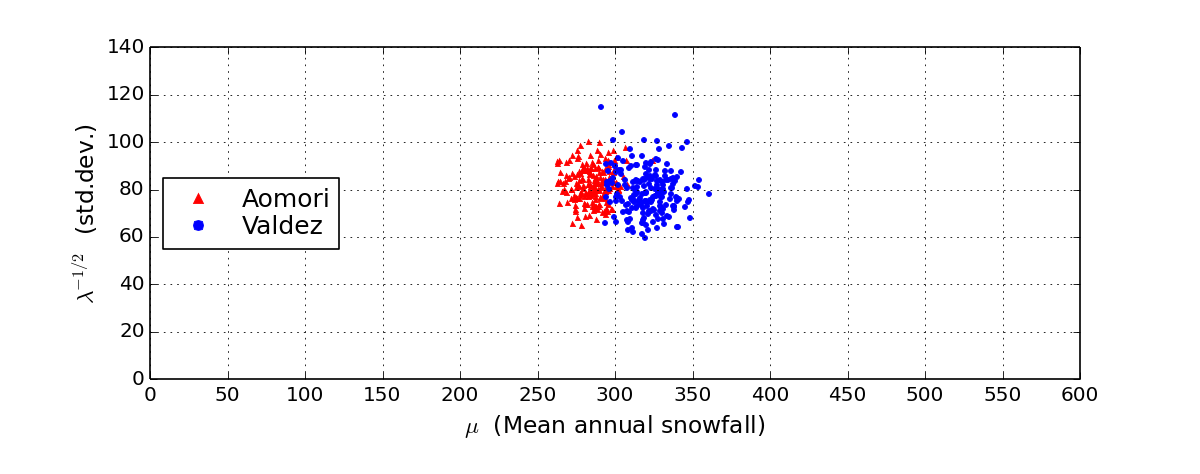
\includegraphics[width=1\textwidth]{code/snow-posteriors-1.png}
    % Source: Original work by J. W. Miller.
  \end{center}
  \caption{Scatterplot of samples from the posteriors for Aomori and Valdez.}
  \label{figure:snow-posteriors}
\end{figure}

See Figure \ref{figure:snow-posteriors} for a scatterplot of samples from each of the posteriors. Visually, the posterior does indeed seem to favor Valdez as having higher mean snowfall. Using $10^6$ samples from each posterior, I approximate the posterior probability that Valdez has higher mean snowfall than Aomori to be:
$$\Pr(\bm\mu_V > \bm\mu_A\mid x_{1:n_A},y_{1:n_V}) \approx 0.987$$
where $x_{1:n_A}$ is the Aomori data and $y_{1:n_V}$ is the Valdez data.



\subsection*{Exercise 5}

I tried the following three different settings of hyperparameters, varying $m$, $b$, and $a$ separately:
\begin{align*}
 & m=500,c=1,a=1/2,b=80^2 a\\
 & m=200,c=1,a=1/2,b=20^2 a\\
 & m=200,c=1,a=10/2,b=80^2 a
\end{align*}
This gave the following three values for the posterior probability that Valdez has higher mean snowfall than Aomori:
\begin{align*}
0.989 \\
0.987 \\
0.987 
\end{align*}
This suggests that the result does not depend that strongly on the choice of prior.  (A more in-depth sensitivity analysis would be needed to verify this.) See Figure \ref{figure:snow-posteriors-alt}.


\begin{figure}
  \begin{center}
    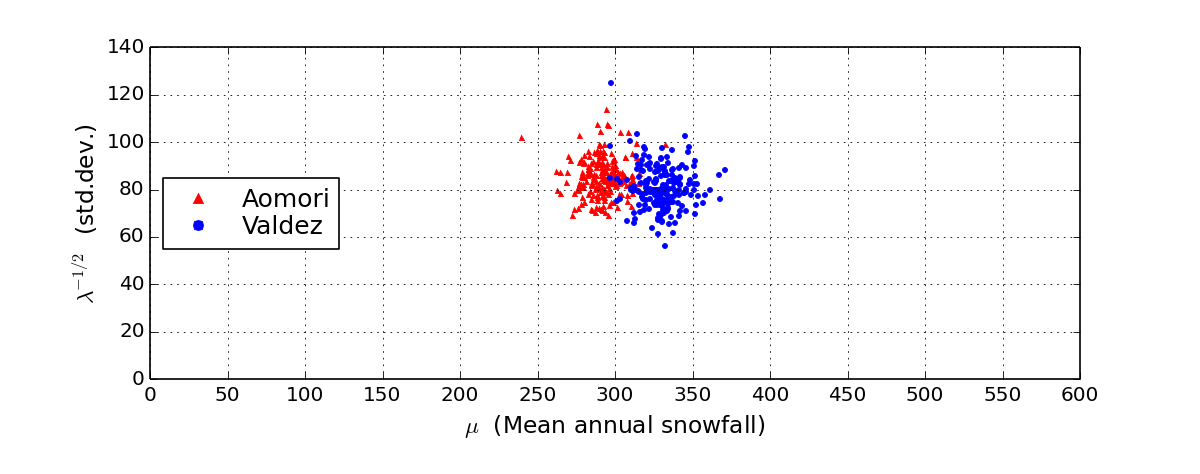
\includegraphics[width=1\textwidth]{code/snow-posteriors-2.png}
    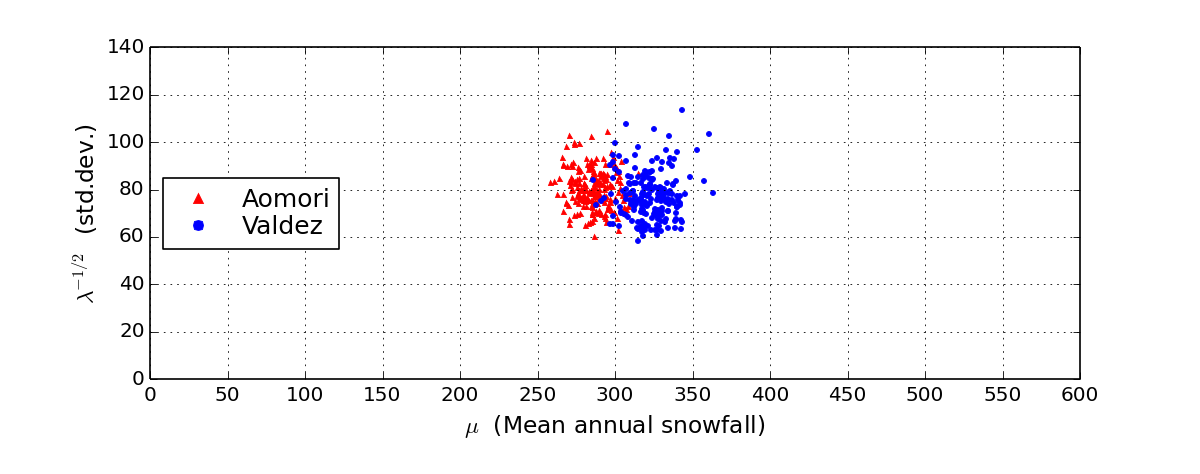
\includegraphics[width=1\textwidth]{code/snow-posteriors-3.png}
    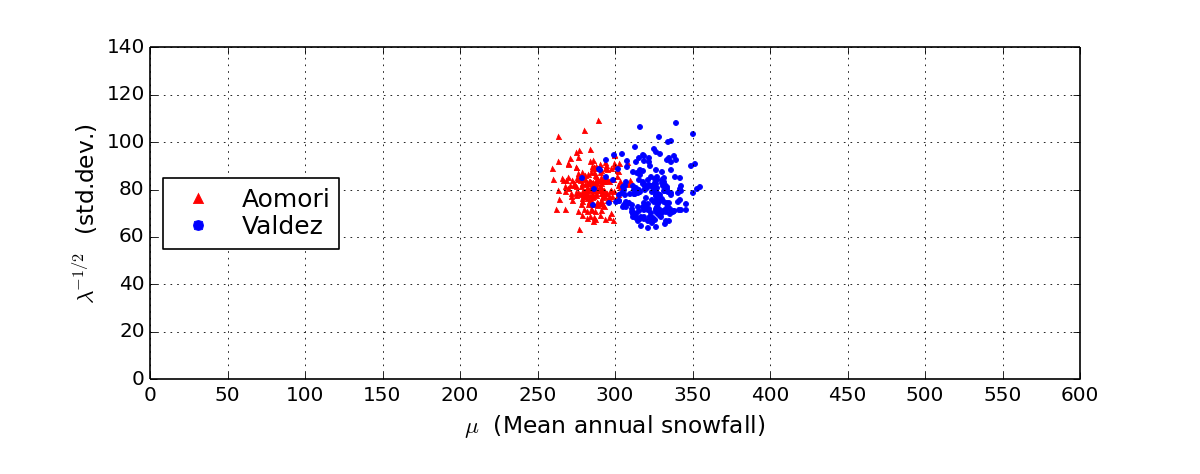
\includegraphics[width=1\textwidth]{code/snow-posteriors-4.png}
    % Source: Original work by J. W. Miller.
  \end{center}
  \caption{Scatterplots of samples from the posteriors for Aomori and Valdez, for the three different choices of hyperparameters.}
  \label{figure:snow-posteriors-alt}
\end{figure}

There is enough data that we would have make the prior extremely different in order to get a significantly different result.
This can be quantified more precisely by looking at how the posterior parameters $M, C, A, B$ depend on $m,c,a,b$, the sample size, and the summary statistics of the data.


\newpage
\appendix
\section{Source code in Julia language}

\subsection*{Exercise 2}
\lstinputlisting[language=julia,numbers=none,commentstyle=\tt\color{OliveGreen}]{code/snow-solution.jl}



\end{document}






